\documentclass{article}
\usepackage{microtype}
\usepackage[utf8]{inputenc} 
\usepackage[a4paper, total={6in, 9.6in}]{geometry}
\usepackage{MnSymbol}
\usepackage{enumerate}
\usepackage{amsmath}
\usepackage{fancyhdr}
\usepackage{xcolor}
\usepackage{tikz}
\usepackage{pgfplots}
\usepackage{marvosym}

\widowpenalties=4 10000 10000 150 0

%% headers
\pagestyle{fancy}
\fancyhf{}
\rhead{Kommunikationssysteme WS19/20}
\lhead{Daniel Schubert, Anton Lydike}
\rfoot{Seite \thepage}

% simple command to display Aufgabe <num>)       ___ / <num>p.
\newcommand\task[1]{\section*{Aufgabe #1)\hfill \underline{\,\,\,\,\,\,}\,\,/1p.}}

% Interpretation (I)
\newcommand\I{I}
% Interpretation und belegung (I, \beta)
\newcommand\Ib{\I, \beta}

%% models
\newcommand\lmodels{\leftmodels} 			% =|
\newcommand\bimodels{\leftmodels\models}	% =||=


%% table for total points
\newcommand\pointsttl[1]{\section*{Gesamtpunkte: \hfill \underline{\,\,\,\,\,\,}\,\,/#1p.}}

%% Funktionen und Prädikate
% Funktionen (arg ist anzahl der stellen)
\newcommand\func[1]{\mathcal{F}^{#1}}
% Prädikate (arg ist anzahl der stellen)
\newcommand\praed[1]{\mathcal{P}^{#1}}

%% Regeln
\newcommand\defrule[2]{\frac{#1}{#2}}

%% Funktionszahl
\newcommand\funcnum[1]{\#_{F}\, #1}

% Für ersetzungen in belegungen wie { x \mapsto d }
\newcommand\repl[2]{\{#1 \mapsto #2\}}

% für alle x .
\newcommand\fall[1]{\forall #1 \, . \,}
\newcommand\ex[1]{\exists #1 \, . \,}

% short biimplication
\newcommand\biimpl{\Leftrightarrow}

% draw a box on the right side of the page
\newcommand\qed{ \hfill $\Box$ }

% red, green, blue text:

\definecolor{greeen}{RGB}{34,139,34}

\newcommand\red[1]{\textcolor{red}{#1}}
\newcommand\green[1]{\textcolor{greeen}{#1}}
\newcommand\blue[1]{\textcolor{blue}{#1}}

% more symbols: https://oeis.org/wiki/List_of_LaTeX_mathematical_symbols

\newcommand\cfgtitle[1]{\title{\vspace{-1.5cm}Übungsblatt #1\\%
\begin{large} Übungsgruppe Metcalfe \end{large}} \lfoot{Übungsblatt #1}\cfoot{Übungsgruppe Metcalfe}}
\author{Daniel Schubert\\Anton Lydike}


%%%%%%%%%%%%%%%%%%%%%%%
%% plotting helpers  %%
%%%%%%%%%%%%%%%%%%%%%%%

%% these draw vertical features
\newcommand\htl[1]{(#1,1) (#1,-1)}  		%% draw line from low to high
\newcommand\lth[1]{(#1,-1) (#1,1)}			%% draw line from high to low

\newcommand\sigtick[2]{\htl{#1} \lth{#2}}	%% draw a htl and then lth line

%% these draw horizontal features
\newcommand\sig[3]{(#2,#1) (#3,#1)}		%% draw a line at height #1 from x=#2 to x=#3
\newcommand\sighi[2]{\sig{1}{#1}{#2}}		%% draw a high signal from #1 to #2
\newcommand\sigmed[2]{\sig{0}{#1}{#2}}		%% draw a null signal from #1 to #2
\newcommand\siglo[2]{\sig{-1}{#1}{#2}}		%% draw a low  signal from #1 to #2


\newcommand\fakeaxis[2]{\addplot [-stealth,black] coordinates {(#1,0) (#2,0)};}



%% units
\newcommand\m{\text{ m}}
\newcommand\s{\text{ s}}
\newcommand\mps{\frac{\text{m}}{\text{s}}}
\newcommand\Gbps{\text{ Gbps}}
\newcommand\bps{\text{ bps}}
\newcommand\bit{\text{ b}}
\newcommand\B{\text{ B}}


\cfgtitle{4}
\date{Mittwoch 20.11.2019}


\renewcommand{\L}{\text{L}}
\newcommand{\R}{\text{R}}
\newcommand\Ssend{\text{S}_{\text{send}}}
\newcommand{\bits}{\text{ b}}

\renewcommand{\iff}{\Leftrightarrow}

\begin{document}
\maketitle
\thispagestyle{fancy}

\task{1}
    
    Wir verwenden folgende Markierungen: Escape-Sequenzen in \green{Grün} und Flags in \blue{Blau}.
    
    \begin{enumerate}[a)]
        \item 
            Jede beliebiebe Bit-Zeichen-Kombination der darüberliegenden Schicht L3 muss sich in den Nutzdaten übertragen lassen. Nutzdatensymbole $\neq$ Steuersymbole.            
        \item 
            \begin{itemize}
                \item Richtig
                \item Falsch
                \item Falsch, ESC-Bytes werden verwendet um flags im Nutzdatenfeld zu kodieren
                \item Falsch, Bit-Stuffing ist eine Art Steuerzeichen in den Nutzdaten zu kodieren und fügt nach $n$ aufeinanderfolgenden einsen eine null ein.
            \end{itemize}
        \item \texttt{\blue{01111110} 0011111\green{0}0011111\green{0}10 \blue{01111110}} 
        
        \item \texttt{\blue{01111110} 01000001 \green{01111101} 01111101 01000010 \green{01111101} 01111110 \blue{01111110}}
    \end{enumerate}
    
\task{2}    

    \begin{enumerate}[a)]
        \item 
        \begin{itemize}
            \item Falsch
            \item Richtig
            \item Falsch
        \end{itemize}
    
        \item 
        
        \textbf{Berechnung der Checksumme:}
        \begin{align*}
            \texttt{ 101101100000} &: \texttt{10011} && = \\
            \underline{\texttt{:10011~~~~~~~}} &                  && = \texttt{1} \\ 
            \texttt{=0010111~~~~~} &                  && = \texttt{10} \\
            \underline{\texttt{  :10011~~~~~}} &                  && = \texttt{101} \\ 
            \texttt{  =0010000~~~} &                  && = \texttt{1010} \\
            \underline{\texttt{    :10011~~~}} &                  && = \texttt{10101} \\ 
            \texttt{    =00011000} &                  && = \texttt{1010100} \\
            \underline{\texttt{       :10011}} &                  && = \texttt{10101001} \\
            \texttt{       =01011} &                  && = \texttt{10101001} \\
     \texttt{Checksumme ist 01011} &                  && = \texttt{10101001} \\
        \end{align*}
        \textbf{Gesicherte Bitfolge:}
        
        \texttt{1011 0110 01011}
        
        \item Empfänger teilt durch Checksumme und kann anhand des Restes sehen, ob Übertragung erfolgreich war.
        
    \end{enumerate}

\task{3}

\begin{enumerate}[a)]
	\item \textbf{ARQ Selective-Repeat:}
		
		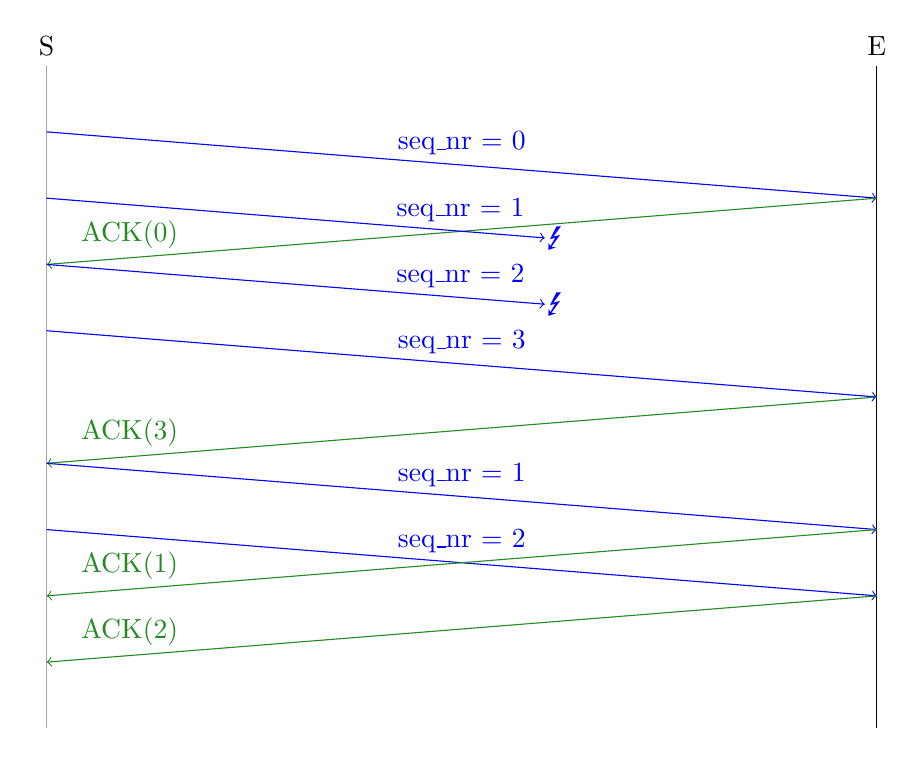
\begin{tikzpicture}
	        \begin{axis}[
	          domain=0:1,
	          xmin=0, xmax=1,
	          ymin=0, ymax=10,
	          axis y line*=left,      
	          axis x line*=top,
		      x axis line style={draw=none},
		      y axis line style={draw=none},
	          height=10cm, width=1\textwidth,
	          xticklabels={S,E},
	          xtick={0,1},
	          tick style={draw=none},
	          yticklabels={}
	          ]
	          
			\addplot [black] coordinates {
				(0,10) (0,0)
			};
			\addplot [black] coordinates {
				(1,10) (1,0)
			};
		          
			\addplot [->,blue] coordinates {
				(0,9) (1,8)
			} node[above,pos=.5] {seq\_nr = 0};
			\addplot [->,greeen] coordinates {
				(1,8) (0,7)
			} node[above,pos=.9] {ACK(0)};

			\addplot [->,blue] coordinates {
				(0,8) (0.6,7.4)
			} node[above,pos=.831] {seq\_nr = 1} node[pos=1.02] {\large{\Lightning}};
			
			\addplot [->,blue] coordinates {
				(0,7) (0.6,6.4)
			} node[above,pos=.831] {seq\_nr = 2} node[pos=1.02] {\large{\Lightning}};
			
			\addplot [->,blue] coordinates {
				(0,6) (1,5)
			} node[above,pos=.5] {seq\_nr = 3};
			\addplot [->,greeen] coordinates {
				(1,5) (0,4)
			} node[above,pos=.9] {ACK(3)};
			
			
			\addplot [->,blue] coordinates {
				(0,4) (1,3)
			} node[above,pos=.5] {seq\_nr = 1};
			\addplot [->,blue] coordinates {
				(0,3) (1,2)
			} node[above,pos=.5] {seq\_nr = 2};
			
			\addplot [->,greeen] coordinates {
				(1,3) (0,2)
			} node[above,pos=.9] {ACK(1)};
			\addplot [->,greeen] coordinates {
				(1,2) (0,1)
			} node[above,pos=.9] {ACK(2)};			
			
		\end{axis}
    	\end{tikzpicture}
    	\item 
    	
    	\begin{itemize}
    		\item $n=3$
    		\item Da 5 rahmen überprüft werden müssen, muss bis 5 gezählt werden. Dafür sind 3 bits notwendig.
    	\end{itemize}
    	
    	\item Das Bandbreite-Verzögerungs-Produkt (bandwidth-delayproduct) wird aus der Bandbreite un der Ausbreitungszeit berechnet. $$\text{BDP}=t_{\text{ausbreitung}} \cdot \text{R}$$
    	\item Da Verarbeitungszeit vernachlässigbar ist, ergibt sich folgende formel für die gesamte Übertragungszeit in abhängigkeit der Rahmenlänge L (in bits):
    	
    	$$ t_\text{send} = \frac{\L}{1\Gbps} = \frac{\L}{10^9\bps} $$
    	
    	Wir wollen nun, dass wir 80\% prozent der zeit senden, also dass das verhältnis von Sendezeit $t_\text{send}$ zu Wartezeit $t_\text{wait} = 2 \cdot D/v = 10^{-6}\s$ größer als $0.8$ ist.
    	\begin{align*}
    		\frac{\R \cdot t_\text{send}}{\R \cdot t_\text{wait}} > 0.8 & \iff \frac{\frac{\L}{10^9\bps}}{10^{-6}\s} > 0.8\\
    		& \iff \frac{\L}{10^3\bits} > 0.8 \\
    		& \iff \L > 0.8 \cdot 10^3 \bits = 800\bits = 100 \text{  B}  
    	\end{align*}
    	
		    	
    	
\end{enumerate}

\pointsttl{3}


\end{document}
